%% Classe du document
\documentclass[a4paper,10pt]{article}

%% Francisation
\usepackage[francais]{babel} % Indique que l'on utilise le francais
\usepackage[T1]{fontenc}
\usepackage[utf8]{inputenc} % Indique que l'on utilise tout le clavier
%\usepackage[latin1]{inputenc}

%% Réglages généraux
\usepackage[top=3cm, bottom=3cm, left=3cm, right=3cm]{geometry} % Taille de la feuille
\usepackage{lastpage}

%% Package pour le texte
\usepackage{soul} % Souligner
\usepackage{color} % Utilisation de couleurs
\usepackage{hyperref} % Créer des liens et des signets
\usepackage{eurosym}% Pour le symbole euro
\usepackage{fancyhdr}% Entête et pied de page

%% Package pour les tableaux
\usepackage{multirow} % Colonnes multiples
\usepackage{cellspace}
\usepackage{array}

%% Package pour les dessins
\usepackage{pstricks}
\usepackage{graphicx} % Importer des images
\usepackage{pdftricks} % Pour utiliser avec pdfTex
\usepackage{pst-pdf} % Pour utiliser avec pdfTex
\usepackage{pst-node} % Pose de noeuds
\usepackage{subfig}
\usepackage{float}

%% Package pour les maths
\usepackage{amsmath} % Commandes essentielles
\usepackage{amssymb} % Principaux symboles

%% Package pour le code
\usepackage{listings} % Utilisation de la couleur syntaxique des langages
\usepackage{url}


\usepackage[babel=true]{csquotes} % Permet les quotations (guillemets)
\usepackage{tocvsec2}
\usepackage{amsthm}
\usepackage{amsfonts}

\usepackage{tikz}
\usepackage{pdfpages}

\usetikzlibrary{shapes} % A revoir

%--------------------- Autres définitions ---------------------%

% Propriété des liens
\hypersetup{
colorlinks = true, % Colorise les liens
urlcolor = blue, % Couleur des hyperliens
linkcolor = black, % Couleur des liens internes
}

\definecolor{grey}{rgb}{0.95,0.95,0.95}

% Language Definitions for Turtle
%TODO: a revoir avec les couleur de gedit
\definecolor{olivegreen}{rgb}{0.2,0.8,0.5}
\definecolor{grey2}{rgb}{0.5,0.5,0.5}
\lstdefinelanguage{ttl}{
sensitive=true,
morecomment=[s][\color{grey2}]{@}{:},
morecomment=[l][\color{olivegreen}]{\#},
morecomment=[s][\color{red}]{<}{/>},
morestring=[s][\color{olivegreen}]{<http://w}{\#>},
morestring=[b][\color{blue}]{\"},
}

\lstset{
frame=single,
breaklines=true,
basicstyle=\ttfamily,
backgroundcolor=\color{grey},
basicstyle=\scriptsize,
keywordstyle=\color{blue},
commentstyle=\color{green},
stringstyle=\color{red},
identifierstyle=\color{blue}
}

%Definition de la commande pour retirer l'espace devant les ':'
\makeatletter
\@ifpackageloaded{babel}%
        {\newcommand{\nospace}[1]{{\NoAutoSpaceBeforeFDP{}#1}}}%  % !! double {{}} pour cantonner l'effet à l'argument #1 !!
        {\newcommand{\nospace}[1]{#1}}
\makeatother

\setcounter{tocdepth}{3}
%\maxsecnumdepth{subsubsection} % Dernière section numérotée

\newcommand{\paperPrototyping}{\emph{paper prototyping}}

% Corps du document :
\begin{document}

% Définition des entêtes et pieds de page
\fancyhead[LE,CE,RE,LO,CO,RO]{}
\fancyfoot[LE,CE,RE,LO,CO,RO]{}
\fancyhead[LO, LE]{Interface Homme-Machine 2}
\fancyhead[RO,RE]{2012/2013}
\fancyfoot[LO,LE]{Université de \scshape{Nantes}}
\fancyfoot[RO,RE]{Page \thepage \ sur \pageref{LastPage}}
\renewcommand{\headrulewidth}{0.4pt}
\renewcommand{\footrulewidth}{0.4pt}

%\maketitle
\begin{titlepage}

\vspace*{\fill}~
\begin{center}
{\large \textsc{Rapport de Projet}} \\
\vspace{1cm}
{\LARGE Projet : Gestionnaire simple de tâches} \\
\vspace{1cm}
\textbf{Taskinator Android} \\
\vspace{0.3cm}

\includegraphics[height=1cm]{Images/Taskinator.png} 
\includegraphics[height=1cm]{Images/android.png} \\
\vspace{1cm}
COUTABLE Guillaume, RULLIER Noémie \\
\today
\end{center}
\vspace*{\fill}

\vspace{\stretch{1}}
\begin{center}
\noindent 

\includegraphics[height=2.5cm]{Images/universite.png}
\end{center}
\pagebreak
\end{titlepage}

\newpage
\tableofcontents  

% Introduction
\newpage
\pagestyle{fancy}

%%%%%%%%%%%%%%%%%%%%%%%%%%%%%%%%%%%%%%%%%%%%%%%%%%%%%%%%%%%%%%%%%%%%%%%%%%%%%
%%%%%%%%%%  Introduction générale
%%%%%%%%%%%%%%%%%%%%%%%%%%%%%%%%%%%%%%%%%%%%%%%%%%%%%%%%%%%%%%%%%%%%%%%%%%%%%
\section{Introduction}
L'objectif de ce projet fut de développer un gestionnaire simple de tâches. Celui-ci devait permettre de créer des listes de tâches et de suivre l'avancement de celles-ci.

Afin de créer cette application que nous avons appelé \textit{Taskinator}, nous avons établit plusieurs étapes dans l'avancement du projet. Ce rapport présentera ces étapes les unes après les autres.

%%%%%%%%%%%%%%%%%%%%%%%%%%%%%%%%%%%%%%%%%%%%%%%%%%%%%%%%%%%%%%%%%%%%%%%%%%%%%
%%%%%%%%%%  Etape 1
%%%%%%%%%%%%%%%%%%%%%%%%%%%%%%%%%%%%%%%%%%%%%%%%%%%%%%%%%%%%%%%%%%%%%%%%%%%%%
\newpage
\section{Les fonctionnalités}
La première étape fut d'analyser l'ensemble des fonctionnalités que notre application devait proposer. 

\subsection{Fonctionnalités principales}
Voici dans un premier temps les fonctionnalités principales:
\paragraph{Créer une liste:} cette fonctionnalité permet à l'utilisateur de créer une liste vide.
\paragraph{Créer une tâche:} cette fonctionnalité permet à l'utilisateur de créer une tâche.
\paragraph{Supprimer un élément:} cette fonctionnalité permet de supprimer une tâche ou une liste. Cette fonctionnalité est à manipuler avec
précaution, en effet dans le cas d'une liste, la suppression de celle-ci implique aussi la suppression de toutes ses tâches.

\subsection{Fonctionnalités secondaires}
Voici les fonctionnalités secondaires:
\paragraph{Paramètre:} cette fonctionnalité permet à l'utilisateur de modifier le type de l'élément sélectionné. Il pourra par exemple choisir de modifier une liste en liste ordonnée ou en une tâche. Cette fonctionnalité est à manipuler avec précaution, en effet si l'utilisateur décide de transformer une liste en tâche l'ensemble des éléments de la liste seront supprimés. %TODO A voir si on garde ?????
\paragraph{Monter / Descendre:} cette fonctionnalité permet de monter ou descendre une liste ou une tâche. Dans le cas d'une liste, toutes ces tâches sont aussi montées/descendues d'un rang. %TODO A voir si on garde ??????? Dans le cas d'une tâche Est-ce qu'on est limitée à sa liste ou est-ce qu'on autorise un déplacement dans une autre liste ?????
\paragraph{Aperçu:} cette fonctionnalité permet à l'utilisateur d'avoir un aperçu de sa liste, se qui permettra l'affichage d'un nombre plus important de tâches. %TODO A voir si on garde

%%%%%%%%%%%%%%%%%%%%%%%%%%%%%%%%%%%%%%%%%%%%%%%%%%%%%%%%%%%%%%%%%%%%%%%%%%%%%
%%%%%%%%%%  Etape 2
%%%%%%%%%%%%%%%%%%%%%%%%%%%%%%%%%%%%%%%%%%%%%%%%%%%%%%%%%%%%%%%%%%%%%%%%%%%%%
\newpage
\section{Storyboard, \paperPrototyping et Scénarios}

%TODO A voir si on garde le storyboard
\subsection{Storyboard}
Le storyboard permet de montrer à quoi sert l'application. Il utilise les star people de Bill VerPlank. A la fin su storyboard, le personnage atteint son but et est satisfait. Nous avons donc ici créé notre storyboard pour notre application:
\begin{figure}[H]
    \center
%    \includegraphics[width=13.9cm]{Images/storyboard.png}
    \caption{Le storyboard}
\end{figure}

\subsection{Scénarios}
Nous avons imaginé différents scénarios d'utilisation de notre application.
\subsubsection{Scénario 1 - Création/Utilisation/Suppression d'une liste}
Ce premier scénario permet de créer une liste et d'y ajouté des tâches.
\begin{enumerate}
\item{L'utilisateur crée une liste et lui donne un nom \textit{Ski}.}
\item{Il crée ensuite une tâche dans cette liste et lui donne un nom \textit{Bonnet}.}
\item{Il crée ensuite une autre tâche dans cette liste et lui donne un nom \textit{Echarpe}.}
\item{Il souhaite maintenant échanger les tâches \textit{Bonnet} et \textit{Echarpe}, il reste longtemps appuyé sur la tâche \textit{Bonnet} et la glisse un rang plus bas.} %TODO A voir - voir pour les gestures 
\item{L'utilisateur supprime la tâche \textit{Bonnet}.}
\item{L'utilisateur supprime la liste \textit{Ski}. Une popup apparaît pour l'avertir que cette suppression supprimera aussi toutes les tâche de la liste.}
\end{enumerate}

\subsubsection{Scénario 2 - Gestion des listes et sauvegarde}
Ce scénario permet de créer des listes et de les modifiers. Il permet aussi de constater que l'état de l'application est sauvegardé.
\begin{enumerate}
\item{L'utilisateur choisit de créer une liste et lui donne un nom \textit{Course}.}
\item{Il décide ensuite de créer une nouvelle liste et lui donne un nom \textit{Sac de voyage}.}
\item{Il décide ensuite d'inverser ces deux listes, pour cela il reste longtemps appuyé sur la liste \textit{Sac de voyage} et la glisse un rangplus haut.}
\item{L'utilisateur va ensuite supprimer la liste \textit{Course}.}
\item{L'utilisateur va ensuite ouvrir une autre application et revenir sur \textit{Taskinator}. Il peut constater que l'application est ouverte avec l'état dans lequel on l'a quittée.}
\item{Cette fois-ci, l'utilisateur quitte l'application. De même s'il l'a lance à nouveau, celle-ci est ouverte avec le dernier état dans lequel on l'a quittée.}
\end{enumerate}


%%%%%%%%%%%%%%%%%%%%%%%%%%%%%%%%%%%%%%%%%%%%%%%%%%%%%%%%%%%%%%%%%%%%%%%%%%%%%
%%%%%%%%%%  Etape 3
%%%%%%%%%%%%%%%%%%%%%%%%%%%%%%%%%%%%%%%%%%%%%%%%%%%%%%%%%%%%%%%%%%%%%%%%%%%%%
\newpage
\section{L'IHM}

\subsubsection{Choix réalisés (Gestures, ...)}
Dans cette section, nous expliquons les choix effectués et pourquoi nous avons choisi de mettre en place ces solutions:

\begin{itemize}
%TODO A voir est-ce qu'on fait un bouton plus pour les listes et pour les taches on clique sur un champs
%TODO Modifier tout le paragraphe
\item \textbf{Fonctionnalité de création de liste:} nous avons choisi de créer de nouvelles listes en cliquant sur le bouton "+" en bas de l'écran. Un nouvel item apparaît sur la page et possède le focus. L'utilisateur doit seulement donner le nom de cette nouvelle liste. Un nouveau bouton "+" apparaît dans cette liste, il permettra de créer de nouvelles tâches pour la liste.
\item \textbf{Fonctionnalité de création de tâche:} nous avons choisi de créer de nouvelles tâches en cliquant sur le bouton "+" présent sous chaque liste pour ajouter une tâche à la liste correspondante. Lorsque l'utilisateur clique sur ce bouton, un nouvel item de tâche apparaît dans la liste (au-dessus du bouton "+") avec le focus. L'utilisateur doit seulement renseigner le nom de la tâche. Nous avons choisi de procéder ainsi plutôt que de mettre un bouton de création dans l'entête de la liste, pour éviter à l'utilisateur de remonter en haut de la liste à chaque fois qu'il souhaite ajouter une tâche (cela peut vite devenir contraignant).
\item \textbf{Fonctionnalité \textit{Monter} et \textit{Descendre}:} nous avons décidé d'accéder à cette fonctionnalité seulement grâce aux gestures. En effet, il suffit à l'utilisateur de rester longtemps appuyer sur une liste ou tâche et de la glisser à l'endroit voulu.
Attention, lors de l'utilisation de cette fonctionnalité dans une liste ordonnée; si on monte ou descend un élément de tel façon qu'un élément coché se trouve être en dessous d'un élément non coché dans la liste, alors le déplacement ne sera pas activé. (Cette dernière précaution n'a pas été implémentée)
\item \textbf{Fonctionnalité \textit{Supprimer}:} nous avons choisi d'ajouter cette possibilité de suppression sur chaque élément pour que l'utilisateur puisse supprimer plus rapidement. De  plus nous avons décidé de faire apparaître une fenêtre d'avertissement car la suppression d'une liste entraîne la suppression de toutes ses tâches. Pour plus de sécurité, le focus de la validation de la suppression est par défaut sur \textit{Non}. %TODO A revoir si on a un focus sur android
%TODO A revoir si on garde
%\item \textbf{Fonctionnalité \textit{Paramètre}:} nous avons décidé pour cette fonctionnalité (qui peut entraîner la suppression de différents éléments) de faire, également, apparaître une fenêtre d'avertissement. Dans cette fenêtre le focus de la validation du changement est mise à \textit{Non}. On perd cependant un peu de vitesse d'exécution (si l'utilisateur souhaite effectivement bien effectuer ce changement) au profit de plus de sécurité.
\end{itemize}

%TODO a compléter
L'application est tout simplement composée d'une zone réservée à l'affichage de la liste en cours de création et d'une bar d'action. %TODO A revoir car on aura le plus mais est-ce qu'on pourrai pas imaginer par la suite un filtre sur le nom des listes ...
\begin{figure}[H]
%    \center
%    \includegraphics[width=14cm]{Images/mainWindow.png}
    \caption{L'application}
\end{figure}


%TODO Mettre l'image du bouton plus en bas ???
%TODO Menu

\subsection{Affichage des listes et tâches}
Afin d'afficher l'ensemble des listes créées et de leur(s) tâche(s), on a décider d'utiliser ExpandableListView, permettant d'afficher l'ensemble des listes et chacune d'entre elle sa ou ses tâche(s).
La liste est décrite à l'aide du xml list.xml et est représentée par un EditText permettant de donner/modifier le nom de celle-ci et d'un ImageButton permettant d('ajouter la fonctionnalité de suppression de liste.
La tâche est décrite par le fichier task.xml et est représentée par une checkbox, un EditText permettant de taper le nom de la tâche et d'un ImageButton permettant d'ajouter la fonctionnalité de suppression sur la tâche.

%%%%%%%%%%%%%%%%%%%%%%%%%%%%%%%%%%%%%%%%%%%%%%%%%%%%%%%%%%%%%%%%%%%%%%%%%%%%%
%%%%%%%%%%  Etape 4
%%%%%%%%%%%%%%%%%%%%%%%%%%%%%%%%%%%%%%%%%%%%%%%%%%%%%%%%%%%%%%%%%%%%%%%%%%%%%
\newpage
%TODO A modifier par guillaume
\section{Le modèle}
Afin de réaliser cette application nous nous sommes basés sur le modèle suivant dont voici le diagramme de classes:
\begin{figure}[htpb]
%	\center
%	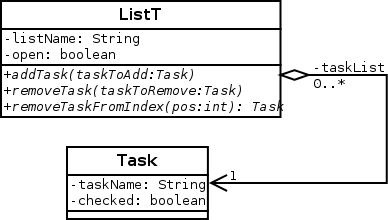
\includegraphics[scale=0.5]{Images/dia_classe.png}
	\caption{Diagramme de classe du modèle}
\end{figure}

Le modèle de cette application est composé d'un pattern composite permettant d'implémenter une structure d'arbre et de composer les différents objets ensemble.
Nous avons donc ici un \textit{Component} qui peut être, soit une \textit{Task} (une tâche), soit une \textit{List} (une liste) qui elle-même peut ensuite être une \textit{SortedList} (une liste ordonnée), celle-ci hérite de la classe \textit{List}. Ce modèle permet donc comme expliqué ci-dessus de composer ces éléments et d'obtenir par exemple des listes de listes de tâches \dots 
Nous pouvons donc gérer tous ces composants au sein de ce modèle et ainsi, ajouter un composant dans une liste, le supprimer, le déplacer d'un rang (dans les deux sens). Nous disposons aussi de toutes les fonctions permettant de déterminer si un composant est cochable ou non.

%%%%%%%%%%%%%%%%%%%%%%%%%%%%%%%%%%%%%%%%%%%%%%%%%%%%%%%%%%%%%%%%%%%%%%%%%%%%%
%%%%%%%%%%  Etape 5
%%%%%%%%%%%%%%%%%%%%%%%%%%%%%%%%%%%%%%%%%%%%%%%%%%%%%%%%%%%%%%%%%%%%%%%%%%%%%
\newpage
\section{Limite de l'application}
Notre application à ses propres limites.
On pourrait imaginer d'ajouter certaines fonctionnalitées comme par exemple:
\begin{itemize}
\item Recherche (
\includegraphics[scale=0.2]{Images/search.png}): qui permetterai à l'utilisateur d'afficher seulement les listes qui ont un nom ou qui ont des tâches dont le nom contient la chaîne du filtre.
\item Partage (
\includegraphics[scale=0.2]{Images/share.png}): qui permettrai à l'utilisateur de partager sa ou ses listes sur des réseaux sociaux ou par mail.
\item Favoris (
\includegraphics[scale=0.2]{Images/favorite.png}): qui permetterai à l'utilisateur de mettre certaines listes ou tâches en favoris et d'y avoir accès via un onglet favoris. Cela permetterai d'avoir un accès plus rapide.
\end{itemize}
%TODO A compléter si des idées A voir si on met tout --> Programmer un rappel d'evenement sur une tâche ajouter un champ information/note

%%%%%%%%%%%%%%%%%%%%%%%%%%%%%%%%%%%%%%%%%%%%%%%%%%%%%%%%%%%%%%%%%%%%%%%%%%%%%
%%%%%%%%%%  CONCLUSION GENERALE
%%%%%%%%%%%%%%%%%%%%%%%%%%%%%%%%%%%%%%%%%%%%%%%%%%%%%%%%%%%%%%%%%%%%%%%%%%%%%
\newpage
\section{Conclusion générale}
Ce projet nous a permis de réfléchir à la structure de l'IHM afin que celle-ci soit la plus intuitive possible pour l'utilisateur. Réfléchir à la position des
boutons, le nom ou l'icône les représentant, comment l'ajout des composants se fera au sein de la liste, la gesture à utiliser, l'utilisation d'un menu \ldots{}
Et donc, d'orienter notre conception sur l'IHM, plus que sur le modèle, et ainsi expérimenter une autre approche de conception.

\end{document}